%%%
%
% $Autor: Wings $
% $Date: 2024-10-31 11:15:45Z $
% $File: file.tex $
% $Version: 1 $
%
% Project: 
%
%%%


\chapter{Entwicklung der Programmlogik}


\subsection{Identifizieren aller Komponenten und Einflussgrößen }
Am Anfang eines jeden Prjektes ist es maßgeblich für den Projekterfolg, alle Komponenten, Parameter und Funktionen eindeutig zu definieren.  Dementsprechend können grafische Übersichten, welche das System aufschlüsseln sinnvoll sein.  
Besonders Mindmaps eignen sich um kategorisch die Komponenten des Systems aufzuzeigen. 

\begin{center}
	\begin{figure}
		%%hier dei xmind \includegraphics{imagefile}
	\end{figure}
\end{center}

\subsection{Entwicklung der Programmlogik }
Um eine effiziente und vorallem eindeutige Verarbeitung von Signalen und Eingaben zu ermöglichen, erweist es sich als sinnvoll eine grafische Übersicht wie ein Flussdiagramm zu erstellen. Diese Grafik kann zudem bei der Programmierung unterstützen. Im Zuge der Entwicklung und Planung eines Systems bietet ein Flussdiagram somit eine strukturierte Darstellung aller relevanten Abläufe und Entscheidungsprozesse. Durch die visuelle Aufbereitung lassen sich komplexe Zusammenhänge leichter nachvollziehen, wodurch sowohl die Implementierung als auch spätere Anpassungen vereinfacht werden.Zusätzlich können potenzielle Fehlerquellen frühzeitig identifiziert und iterativ durch Verbessern der Logik beseitigt werden. Eindeutig dient dieses Diagramm als Blaupause der Programmstruktur und kann somit bereits früh, benötigte Klassen und Funktionen definieren. 
Ein Grafik zur 

\begin{center}
	\begin{figure}
		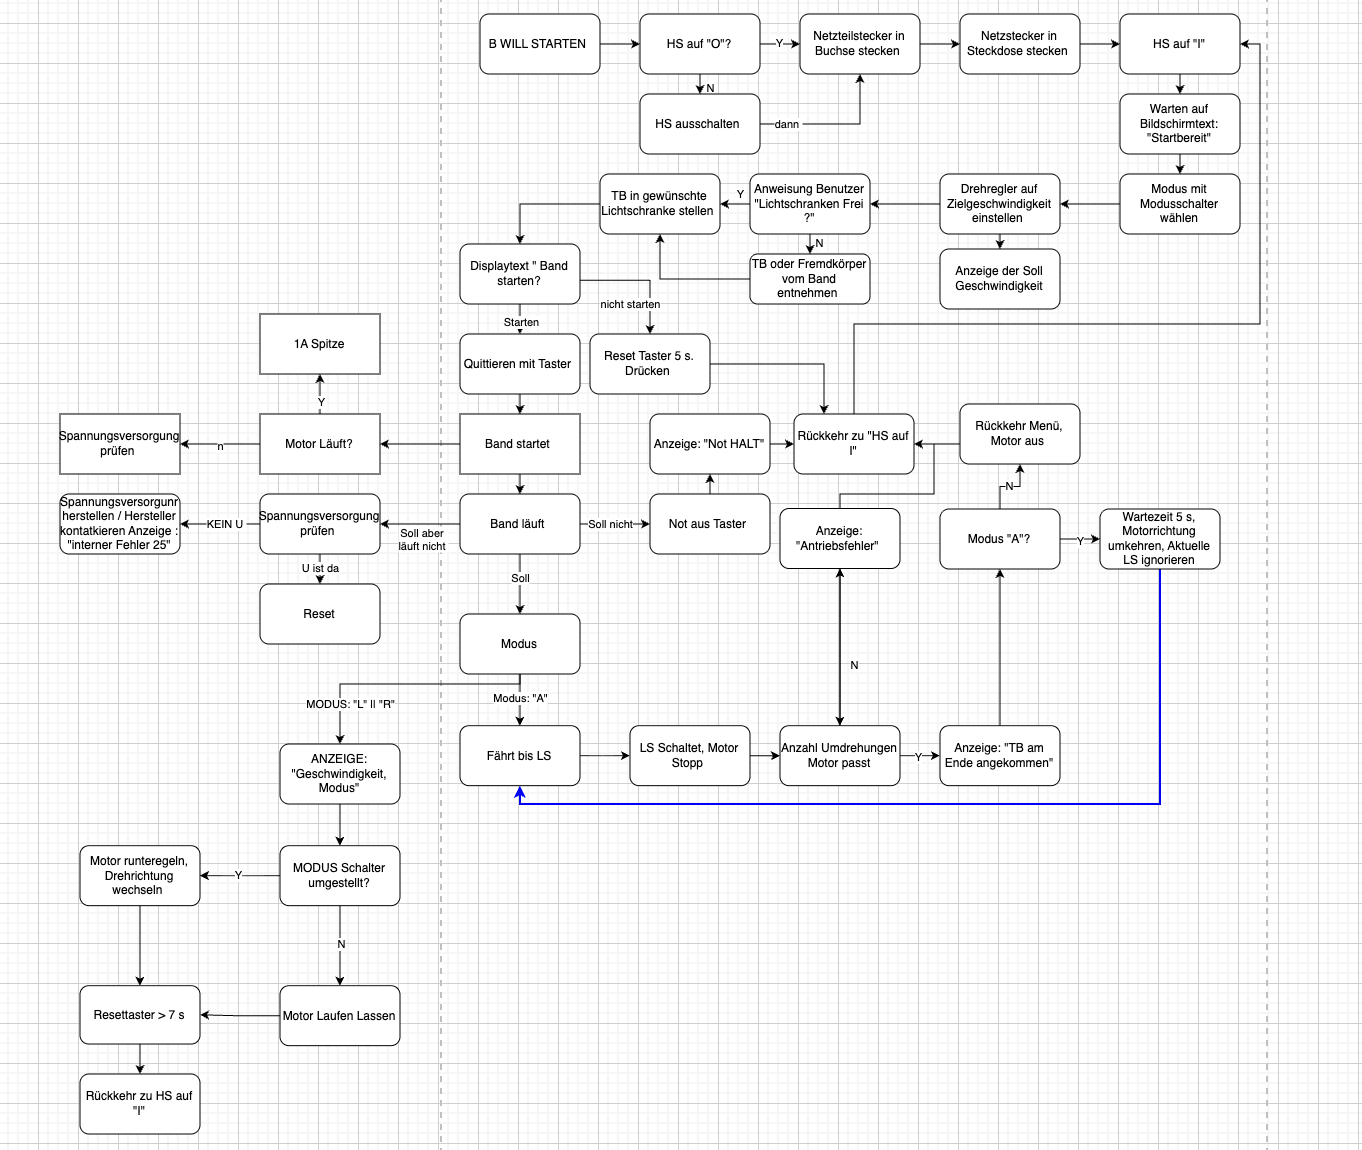
\includegraphics[scale=0.5]{../../Images/General/FlowChartV1.png}
		\caption{Das Erste Flussdiagramm zur Beschreibung des erzielten Programmablaufes}
	\end{figure}
	
\end{center}

